\chapter{Overall Conclusions and Future Directions}

This dissertation develops statistical learning models, generally simpler than mechanistic models, to predict unimpaired flows of California basins from available data. Several issues arise in this prediction problem: 

(1) How we view hydrology, and how we define an observational unit, determines how data is pre-processed for statistical learning methods. So, one issue is in deciding the organizational form of the data (i.e., aggregate vs. incremental basins). Chapter two showed that ``incremental basin'' modeling provides an easy way to include network information in statistical models and the results show its value for modeling hydrology with parametric models, especially those with few parameters like LM and GLM. As the results showed, the LM and GLM prefer the incremental modeling approach, whereas the RF and the NN are somewhat insensitive to it. 

(2) Often, water resources problems are not concerned with accurately predicting the expectation (or the mean) of a distribution, but require estimates of extreme values of the distribution (i.e., floods and droughts). Solving this problem involves defining asymmetric loss functions presented in chapter three. In symmetric loss functions such as the squared error loss functions (i.e., Mean Squared Error or MSE), the peaks or high leverage points get fitted at the expense of the low flows. The proposed Weighted Least Squared Error (WLSE) and Linear-Exponential Error (LINEXE) asymmetric losses are able to force a fit to the tails of the distribution (the peaks and valleys of the hydrograph). The Log-Cosine Hyperbolic Error (LOGCOSH) performs similarly to the Mean Absolute Error (MAE) and MSE. The Mean Squared Percentage Error (MSPE) is chronically biased towards lower predictions and is not suited to problems where the data is skewed positive. In general, the differences show the amount of control the modeler has on the predictions and their probability distribution when picking a loss function.

(3) Hydrologic data are structured, meaning dependencies and correlation structures are inherent in the data (temporal and spatial autocorrelation) and rivers form a network of flows that feed into one another (hierarchical autocorrelation). These characteristics require careful construction of resampling techniques for model error estimation. In chapter four, blocking methods show how much random ones underestimate model error. Models evaluated with random methods have artificially low errors due to the pseudo-replication from autocorrelation. This is not to say that, in hydrology, random resampling is never useful; a random test-train split is most appropriate for predicting flow for a sparsely incomplete gauge record. Blocked resampling in time is most appropriate for predicting or extrapolating streamflow in time for that location. One should not expect to use these resampling strategies and get the same predictive accuracy in a purely ungauged basin problem, where blocks are supposed to be designed across geographic space (or more accurately hierarchical structure). Results show that generally model performance estimates decline as block sizes increase. 

(4) Non-stationarity due to climate change may require adjustments to statistical models, especially if they are meant for long-term decision-making. Chapter five compares unimpaired flow predictions from a statistical model that uses climate variables representing future hydrology to projections from climate models. There is fairly good agreement in the statistical (NN) model's unimpaired flow predictions and the mechanistic (GCM) models routed runoff (R\textsuperscript{2}= [0.64-0.72]). However, the NN model does not capture low flows like the climate models and overestimates their values so much so that when we compare more smoothed data (with a moving average window) we can see a bias emerge ($\beta_1$= [0.95-1.84] for CanESM2 RCP 4.5 for example). This can also be seen in the time series comparisons, where with a larger moving average window the NN model's predictions are systematically higher than the climate model projections.

%-----------------------------------------------------------------------------------------------------------------------------------------------------------------------------------------------------
\section{Model Improvement Strategies}
Figure \ref{fig:modrestime} shows the residuals for the NN model built on observed data in the previous chapters. Model residuals are positive for smaller hierarchies and negative for larger ones. This was evident by the fact that the model over-predicts lower flows (that tend to occur at smaller hierarchies) and under-predicts higher flows (that tend to occur at larger hierarchies). Also, residuals tend to increase with increasing flow (Figure \ref{fig:modresvsflow}), but standardized residuals decrease with flow (Figure \ref{fig:modresvsflowstd}). 

\begin{figure}
	\centering
	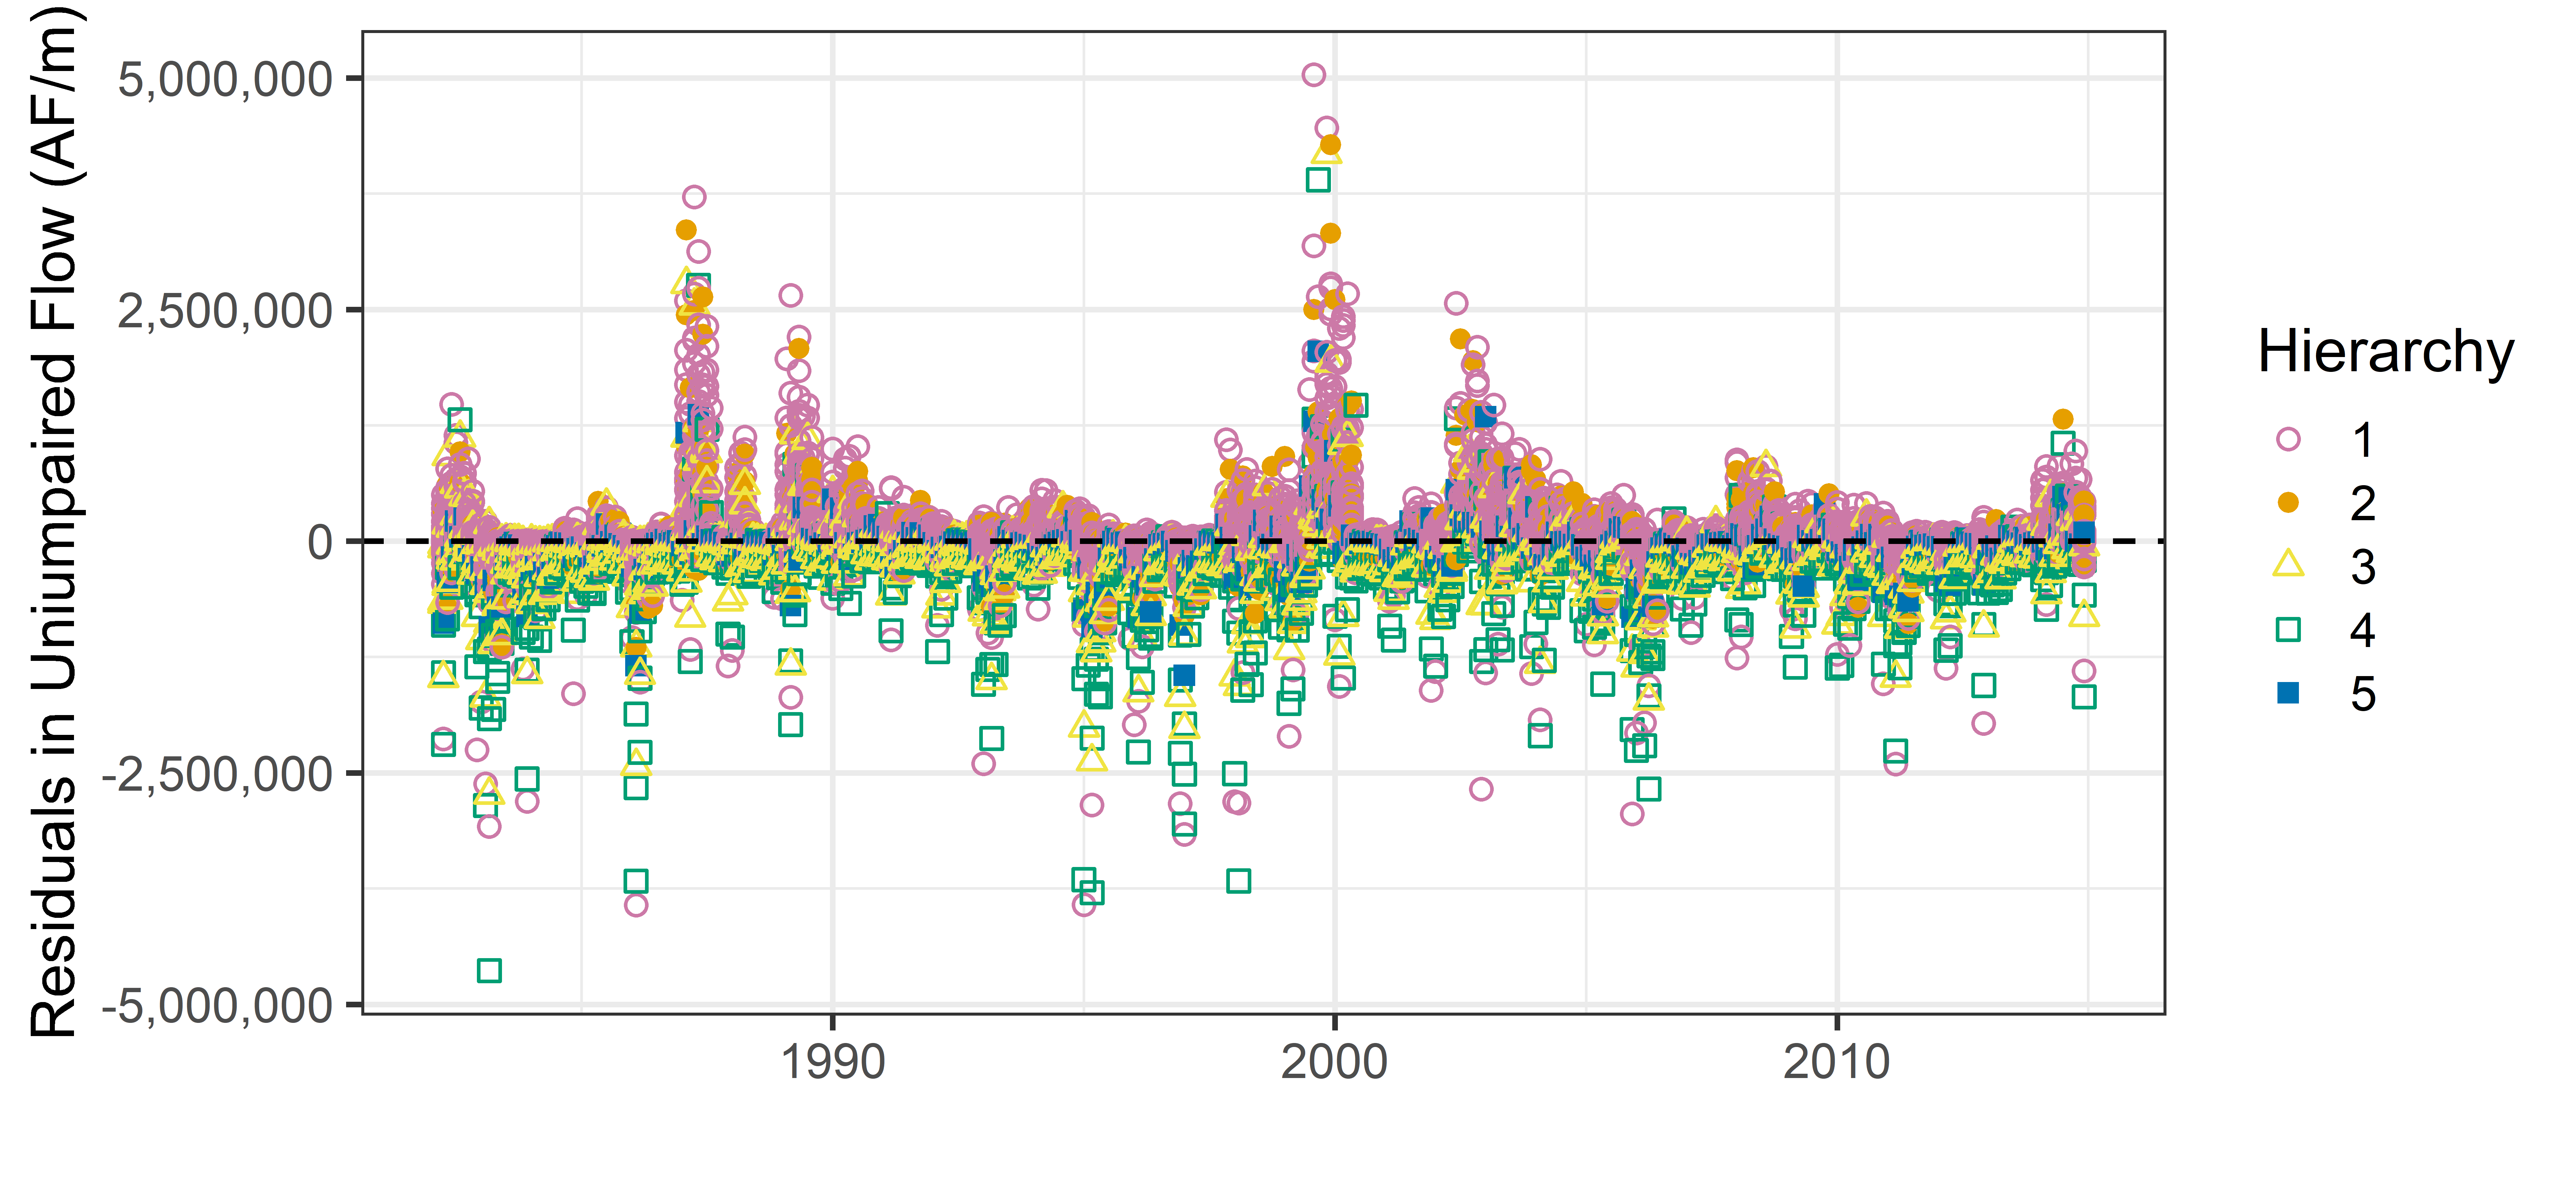
\includegraphics[width=\textwidth,trim={0 0 0 0},clip=true]{plots/rplot51_resovertime.png}
	\caption[NN model residuals over time.]{NN model residuals over time. Residuals may appear random as a whole, however, they tend to be positive for smaller hierarchies and negative for larger ones.} 
	\label{fig:modrestime}
\end{figure}

\begin{figure}
	\centering
	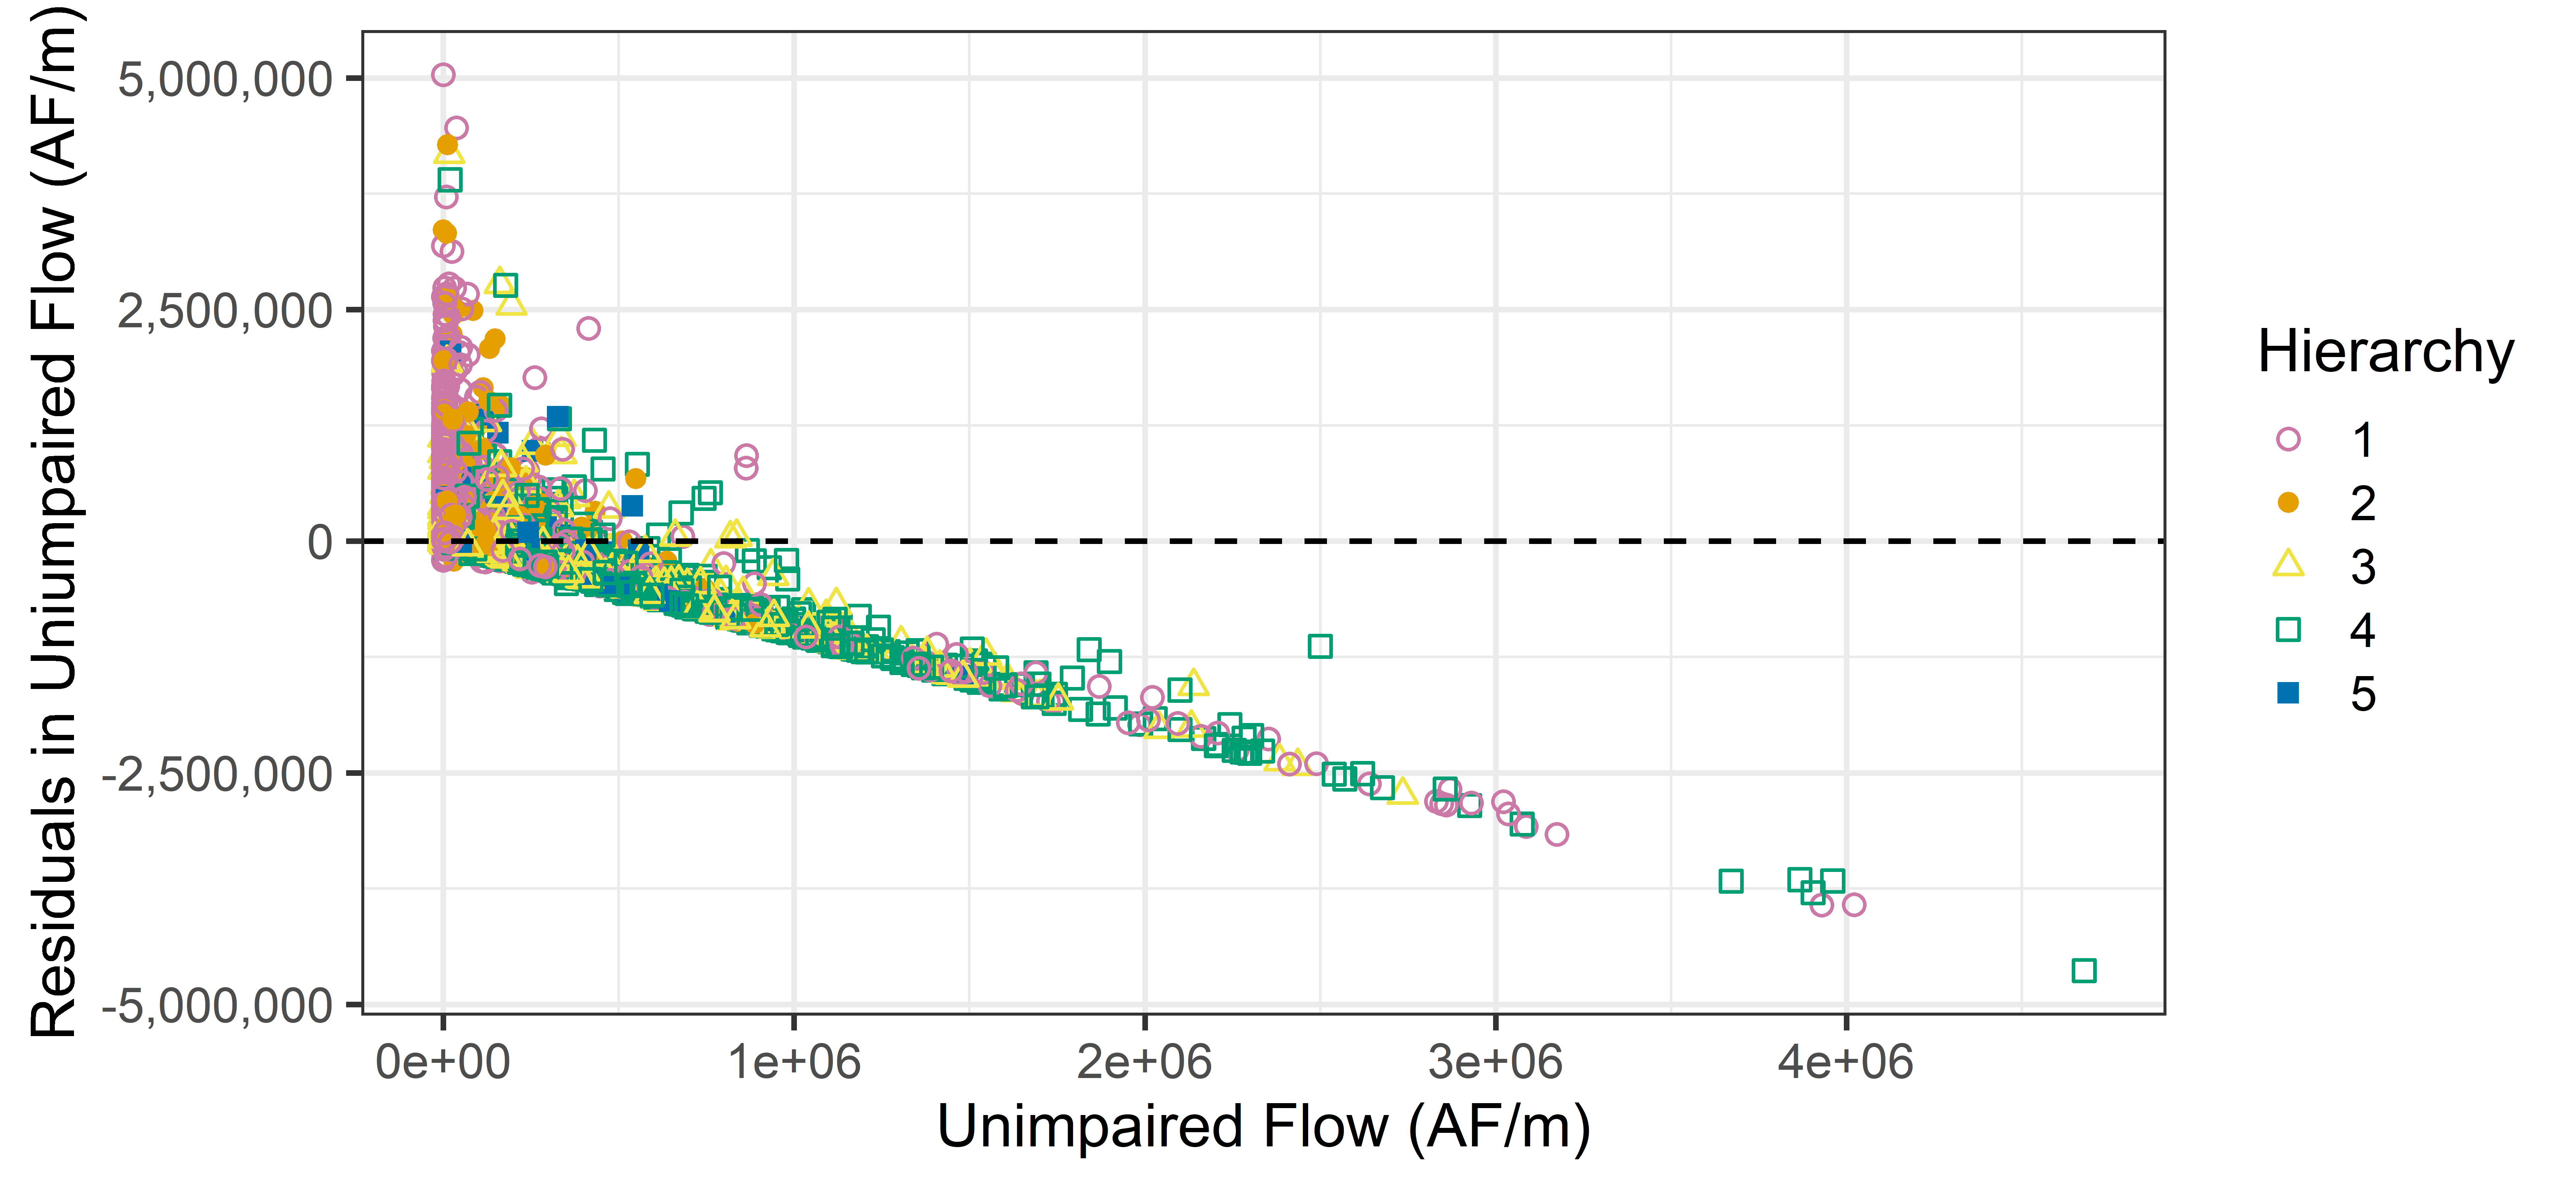
\includegraphics[width=\textwidth,trim={0 0 0 0},clip=true]{plots/rplot51_resvsflow.png}
	\caption[NN model residuals vs. unimpaired flow.]{NN model residuals vs. unimpaired flow. Model residual increase with an increasing response variable. Most of these flows occur at the larger hierarchy (4) as these basins are lower in the network and are expected to have larger flows.} 
	\label{fig:modresvsflow}
\end{figure}

\begin{figure}
	\centering
	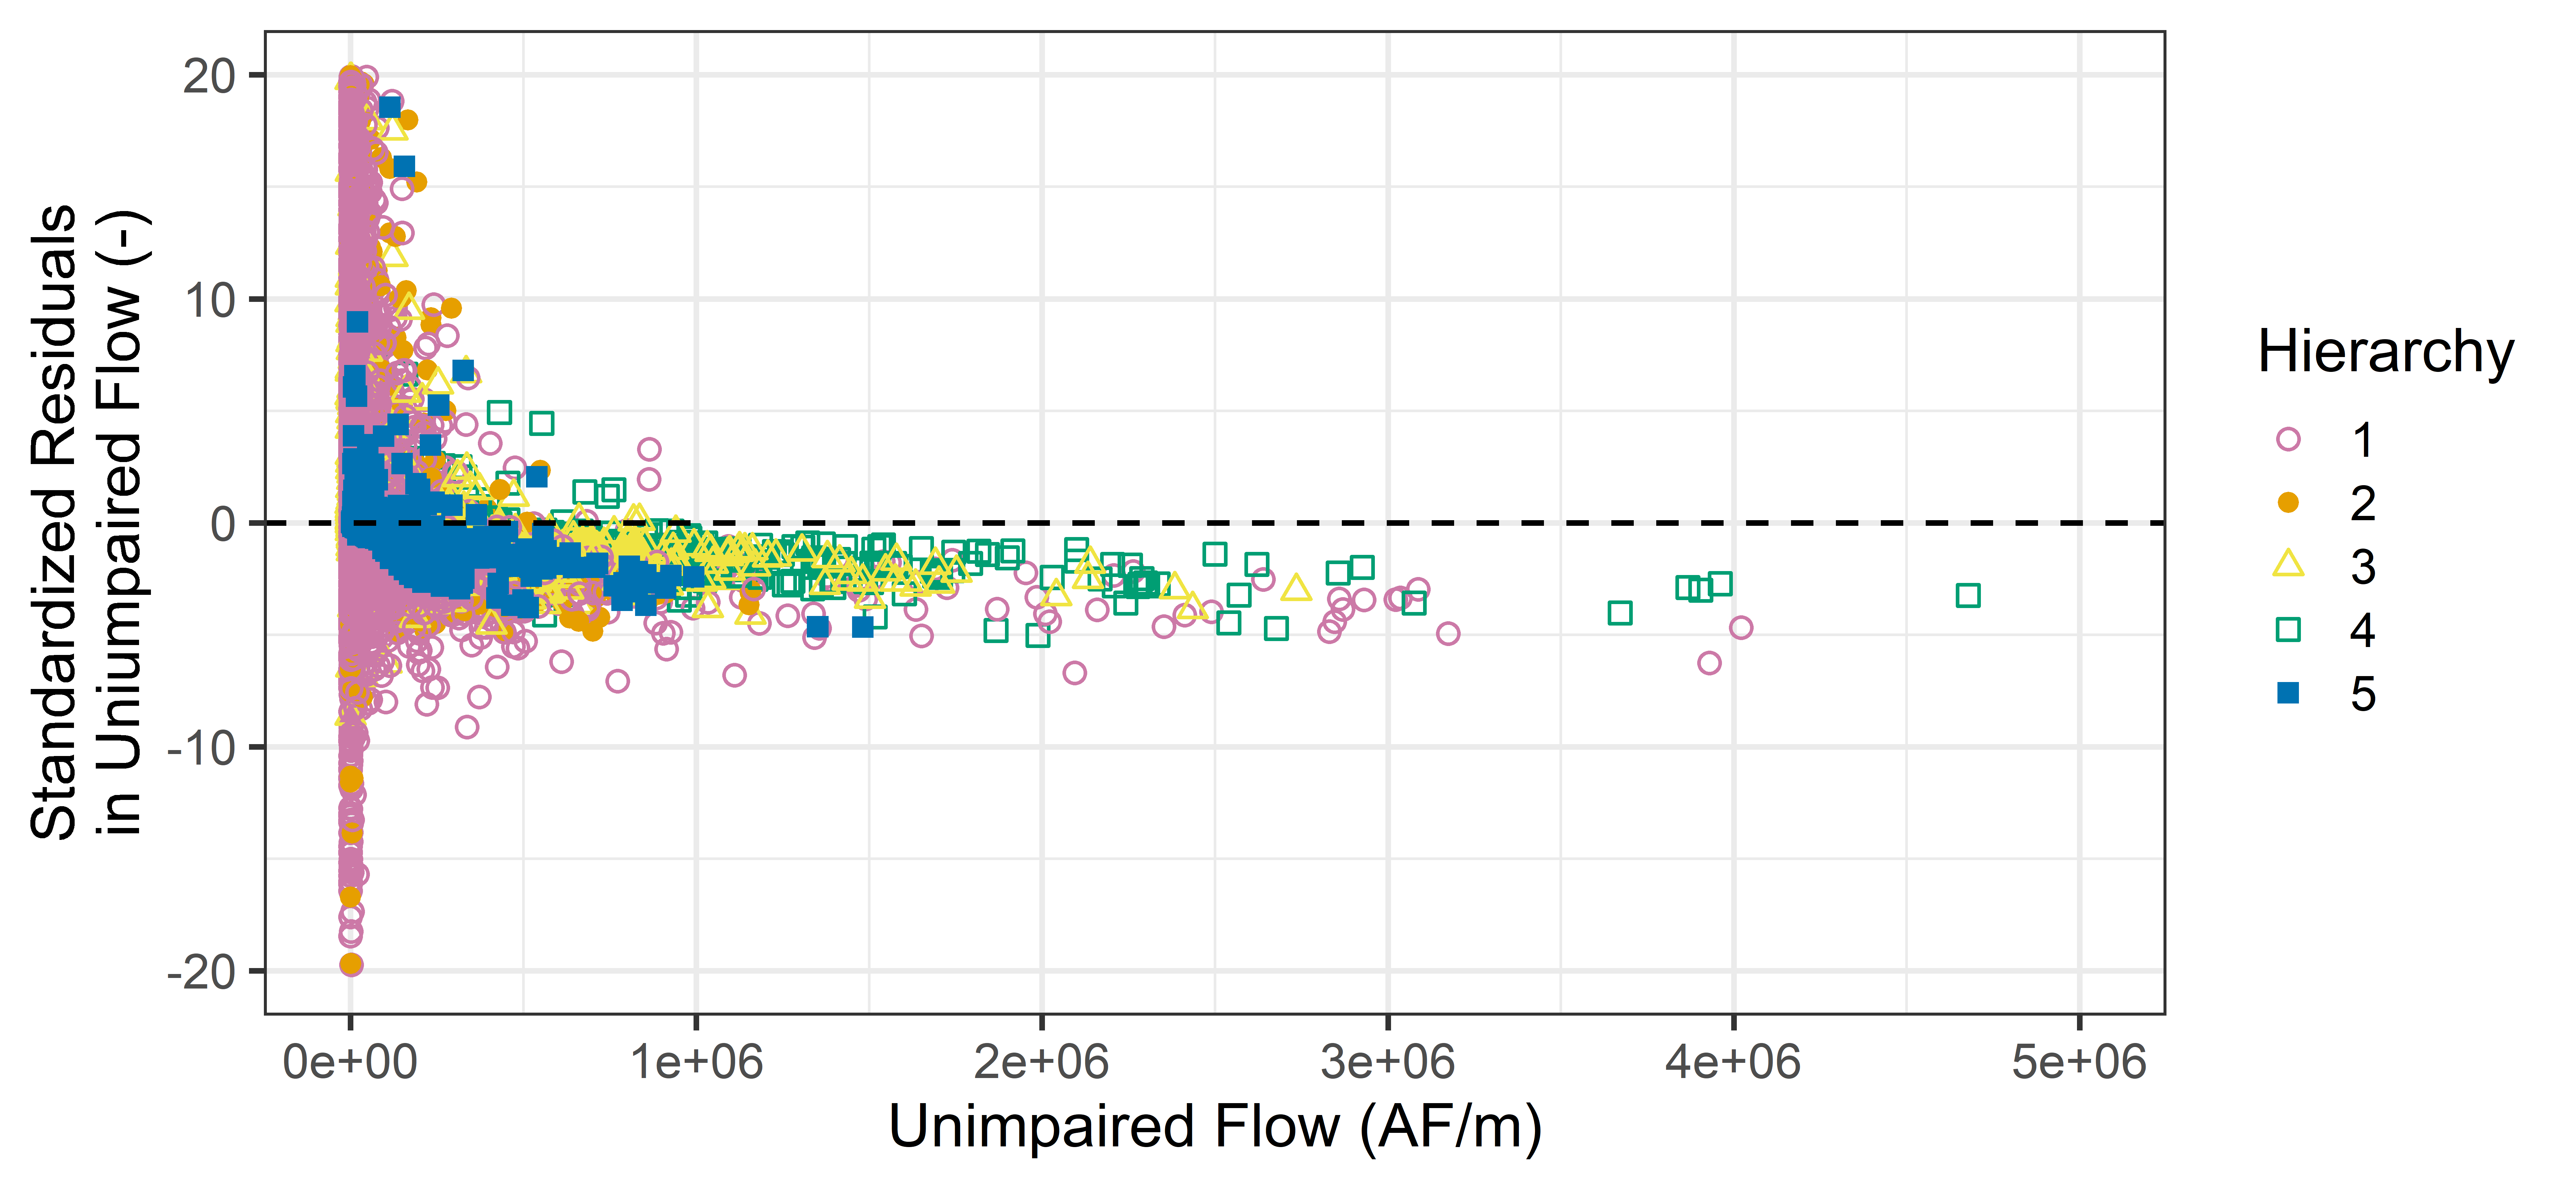
\includegraphics[width=\textwidth,trim={0 0 0 0},clip=true]{plots/rplot51_resvsflow_standardized.png}
	\caption[Standardized NN model residuals vs. unimpaired flow.]{Standardized NN model residuals vs. unimpaired flow. The ratio of model residuals to mean annual observed unimpaired flow decrease with an increasing response variable. Most relative errors occur at smaller hierarchies (1) as these basins are higher in the network and are expected to have smaller flows.} 
	\label{fig:modresvsflowstd}
\end{figure}

Overall, the NN model residuals may appear to be spaced at random. However, with the Box-Pierce and Ljung-Box tests for auto-correlation we can see that in most basins they are not (Figure \ref{fig:bpljtest}). These tests, also known as the ``portmanteau'' tests, are used for examining the null hypothesis of independence in a given time series. P-values close to zero are evidence against independence and imply that the model can be improved to eliminate non-random patterns in the residuals.  

\begin{figure}
	\centering
	\includegraphics[width=\textwidth,trim={0 0 0 0},clip=true]{plots/rplot51_bpljtest.png}
	\caption[Box-Pierce and Ljung–Box tests for auto-correlation in model residuals.]{Box-Pierce and Ljung–Box tests for auto-correlation in model residuals. The p-values close to zero indicate that residuals are auto-correlated. Most basins suffer from 0 p-values indicating that the model can be improved to eliminate non-random patterns in its residuals.} 
	\label{fig:bpljtest}
\end{figure}

Model improvement can come from switching to a model type that focuses on the time series component of the data. For example, some models use a lagged response variable to construct the model as in the Auto Regressive Integrated Moving Average (ARIMA) models. These models are uni-variate. To accommodate for exogenous variables we can use a Seasonal ARIMA (SARIMA). In these models, we have to be careful about introducing information at locations that are supposed to be ungauged and resampling would require eliminating part of the dataset used in modeling. To avoid this problem altogether, we can use models like Recurrent Neural Networks (RNNs) that have the capability of connecting previous information to the present in their architecture. A special type of RNNs, Long Short Term Memory networks (LSTMs) are capable of learning long-term dependencies and would be an excellent next step in improving upon this work. 

Model improvement can also come from a more granular dataset; daily rather than monthly data can increase model performance, since the variable importance plots showed that most information is in precipitation rates and a basin's drainage area. 

In general, rainfall-runoff models can be used inside hydrology, as exploratory research tools, or outside hydrology, for planning, design, or operational decisions. The models developed here are intended for use outside hydrology where hydrologic information is relevant and useful. I started studying the PUB problem during my undergraduate years, because streamflow estimates were needed as a pre-requisite to the original task of estimating nutrient loadings. The model was ultimately intended to inform the Kentucky Division of Water in establishing total maximum daily loads. Like this application, streamflow dis-aggregation and water budget outputs can be used to aid in setting minimum in-stream flow regulations, establishing water rights, modeling river stage-discharge relationships or water levels in a channel, simulating sediment and nutrient loadings, cleaning up anomalies in the data or filling in missing records, and managing natural disasters to name a few. 


